%%%%%%%%%%%%%%%%%%%%%%%%%%%%%%%%%%%%%%%%%%%%%%%%%%%%%%%%%%%%%%%%%%%%%%%%%%%%%%%%%%%%%%%%%%%%%%%%%%
%%%%%%%%%%%%%%%%%%%%%%%%%%%%%%%%%%%%%%%%%%%%%%%%%%%%%%%%%%%%%%%%%%%%%%%%%%%%%%%%%%%%%%%%%%%%%%%%%%
\section{Conclusion and Discussion}
%%%%%%%%%%%%%%%%%%%%%%%%%%%%%%%%%%%%%%%%%%%%%%%%%%%%%%%%%%%%%%%%%%%%%%%%%%%%%%%%%%%%%%%%%%%%%%%%%%
%%%%%%%%%%%%%%%%%%%%%%%%%%%%%%%%%%%%%%%%%%%%%%%%%%%%%%%%%%%%%%%%%%%%%%%%%%%%%%%%%%%%%%%%%%%%%%%%%%
\label{discussion_sec}

In this paper, we proposed an ambitious goal for \aml: the automatic discovery of whole ML algorithms from basic operations with minimal restrictions on form. The objective was to reduce human bias in the search space, in the hope that this will eventually lead to new ML concepts. As a start, we demonstrated the potential of this research direction by constructing a novel framework that represents an ML algorithm as a computer program comprised of three component functions (\setup, \predict, \learn). Starting from empty component functions and using only basic mathematical operations, we evolved neural networks, gradient descent, multiplicative interactions, weight averaging, normalized gradients, and the like. These results are promising, but there is still much work to be done. In the remainder of this section, we motivate future work with concrete observations.

\textbf{The search method} was not the focus of this study but to reach our results, it helped to (1) add parallelism through migration, (2) use FEC, (3) increase diversity, and (4) apply hurdles, as we detailed in Section~\ref{methods_search_sec}. The effects can be seen in Figure~\ref{ablation_comparison_fig}. Suppl.\ Section~\ref{ablation_comparison_thorough_sec} shows that these improvements work across compute scales (today's high-compute regime is likely to be tomorrow's low-compute regime, so ideas that do not scale with compute will be shorter-lived). Preliminary implementations of crossover and geographic structure did not help in our experiments. The silver lining is that the \amlz search space provides ample room for algorithms to distinguish themselves (\eg Section~\ref{difficulty_sec}), allowing future work to attempt more sophisticated evolutionary approaches, reinforcement learning, Bayesian optimization, and other methods that have helped \aml before.

% Source: https://colab.corp.google.com/drive/1rLEVZ-_gGZkX2GFHDHFpz2rTTc_7ePea#scrollTo=ran-8NFqhruP&line=47&uniqifier=1
\begin{figure}[ht]

\begin{centering}
\centerline{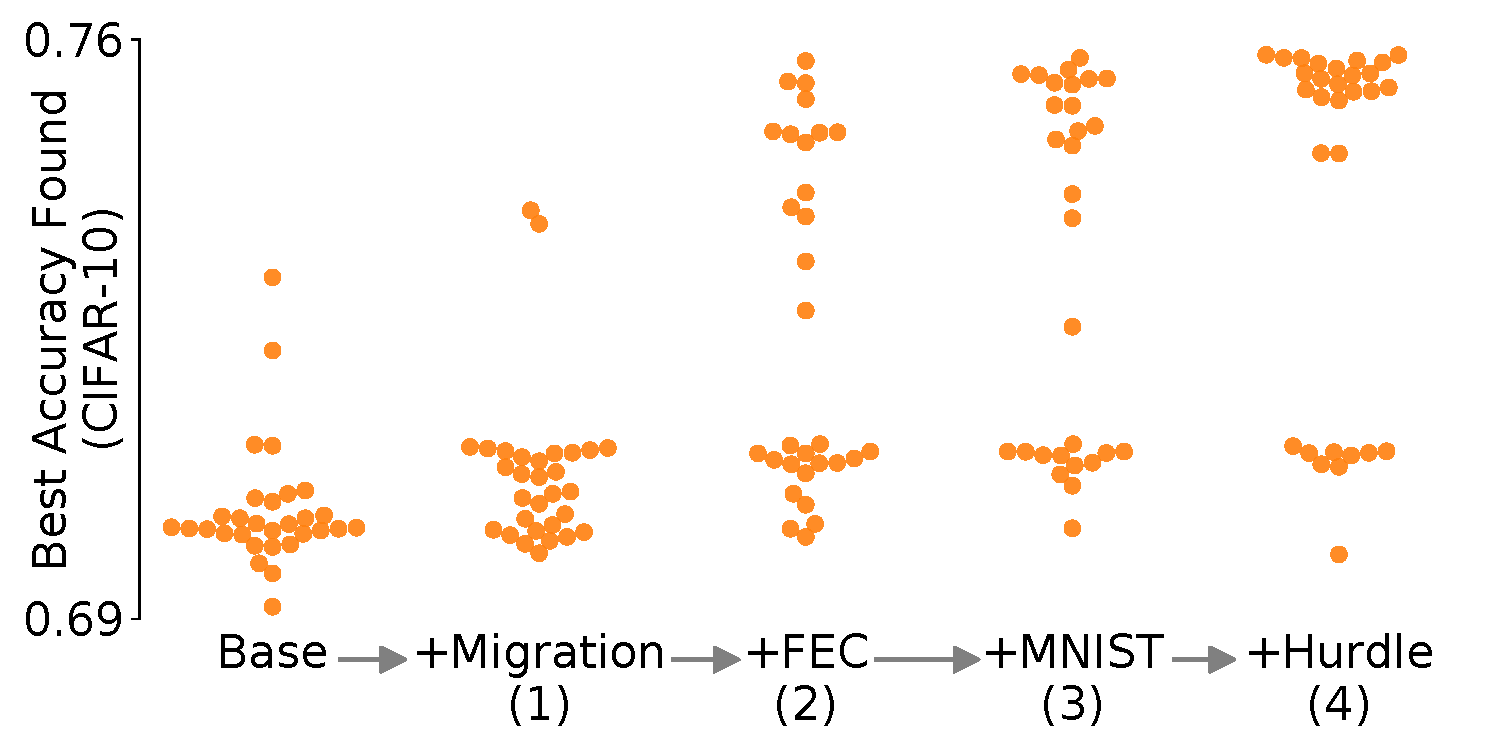
\includegraphics[width=\columnwidth]{ablation_comparison.pdf}}
\caption{Search method ablation study. From left to right, each column adds an upgrade, as described in the main text.}
\label{ablation_comparison_fig}
\end{centering}
\end{figure}

\textbf{Evaluating evolved algorithms} on new tasks requires hyperparameter tuning, as is common for machine learning algorithms, but without inspection we may not know what each variable means (\eg ``Is \textcode{s7} the learning rate?''). Tuning all constants in the program was insufficient due to \textit{hyperparameter coupling}, where an expression happens to produce a good value for a hyperparameter on a specific set of tasks but won't generalize. For example, evolution may choose \textcode{s7=v2$\cdot$v2} because \textcode{v2$\cdot$v2} coincides with a good value for the hyperparameter \textcode{s7}. We address this through manual decoupling (\eg recognizing the problematic code line and instead setting \textcode{s7} to a constant that can be tuned later). This required time-consuming analysis that could be automated by future work. More details can be found in Suppl.\  Section~\ref{reevaluation_supp_sec}. 

\textbf{Interpreting evolved algorithms} also required effort due to the complexity of their raw code (Suppl.\  Section~\ref{interpretation_supp_sec}). The code was first automatically simplified by removing redundant instructions through static analysis. Then, to decide upon interesting code snippets, Section~\ref{zoo_sec} focused on motifs that reappeared in independent search experiments. Such \emph{convergent evolution} provided a hypothesis that a code section may be beneficial. To verify this hypothesis, we used ablations/\emph{knock-outs} and \emph{knock-ins}, the latter being the insertion of code sections into simpler algorithms to see if they are beneficial there too. This is analogous to homonymous molecular biology techniques used to study gene function. Further work may incorporate other techniques from the natural sciences or machine learning where interpretation of complex systems is key.

\textbf{Search space enhancements} have improved architecture search dramatically. In only two years, for example, comparable experiments went from requiring hundreds of GPUs \cite{zoph2017learning} to only one \cite{liu2018darts}. Similarly, enhancing the search space could bring significant improvements to \amlz. Also note that, despite our best effort to reduce human bias, there is still implicit bias in our current search space that limits the potential to discover certain types of algorithms. For instance, to keep our search space simple, we process one example at a time, so discovering techniques that work on batches of examples (like batch-norm) would require adding loops or higher-order tensors. As another case in point, in the current search space, a multi-layer neural network can only be found by discovering each layer independently; the addition of loops or function calls could make it easier to unlock such deeper structures. 
